%-----appendices
\begin{appendices}
\noappendicestocpagenum
\addappheadtotoc
\chapter{Checklist for cooldown}
%-----appendices
\label{appendix:checklist-for-cooldown}


\begin{tabular}{ l r c }
  Date: \underline{\hspace{4cm}} & Name: \underline{\hspace{4cm}}
\end{tabular}

\paragraph{Pump station area - \hef}

\begin{checklist}
 \item flow meters on and working
 \item \{$\Box$ UTL, $\Box$ 500TL, $\Box$ WTL, $\Box$ MTL, $\Box$ 100TL, $\Box$ LTL\} pumped down
 \item \{$\Box$ 250LD, $\Box$ 500LD\} Goddard fittings assembled and ready
 \item 500LD level probe/monitor plugged in and powered on
 \item helium gas cylinder hooked up to 500LD
 \item at least one full backup helium cylinder nearby
 \item dewar scale and weight record form is ready
 \item system is purged and backfilled with helium gas
 \item 500LD is bunged in both LHe inlet and outlet ports
 
\end{checklist}

\paragraph{Pump station area - \het}
\begin{checklist}
 \item \lnn{} trap regenerated
 \item \lnn{} trap filled
 \item vacuum test \het{} lines
 \item record \het{} tank pressures in log book (T$_1$, T$_2$, T$_3$)
 \item flow meter on \het{} gas rack powered on and recording
 \item system is purged and backfilled with helium gas 
\end{checklist}

\paragraph{Gamma Vault}
\begin{checklist}
 \item 100LD Goddard fittings assembled and installed on 100LD
 \item 100LD LHe inlet and outlet ports are bunged
 \item install exhaust tubing on 100LD and point the toward center of GV
 \item \{$\Box$ 100LD LHe, $\Box$ magnet \lnn, $\Box$ magnet LHe\} level sensors reading
 \item fill \lnn{} in magnet space
 \item OVC assembled and pumped down to $\sim$1E-5 mbar %found tilde command from http://www.ctan.org/tex-archive/info/symbols/comprehensive/symbols-a4.pdf
 \item IVC manifold assembled and hooked up to fridge
 \item \het{} section is tight (requires temporary IVC seal)
 \item Lakeshore sensors read to computer
 \item AVS-47 bridge is warmed up and all sensors working
 \item walkie talkies charged
 \item install the 100TL in the 100LD and attach the bayonet to the WTL
 \item fridge heating tapes and tested (geometrically and electronically)
\end{checklist}

\paragraph{Microwaves}
\begin{checklist}
 \item EIO water is running
 \item laptop webcam working
 \item microwaves tested with power meter
 \item wave guide is hooked up to fridge
 \item thermistors and water flow readouts work and read to computer
\end{checklist}

\paragraph{NMR}
\begin{checklist}
 \item signal acheived with oscillator crystal in mixing chamber coil
 \item NMR water is running
 \item PDP running
\end{checklist}


\chapter{SLPM Conversion}
\label{appendix:slpm-conversion}
Some HiFrost documents from CERN refer to flow rates of \hef{} and \het{} in millimoles per second.  The formula to convert this flow rate to SLPM is
\begin{equation}
 \textrm{[SLPM]}=\left(\frac{60\textrm{ s}}{\textrm{min}}\right)\left(\frac{x\textrm{ mol}}{\textrm{s}}\right)\left(\frac{4\textrm{ g}}{\textrm{mol}}\right)\left(\frac{1\textrm{ L}}{0.1785\textrm{ g}}\right)
\end{equation}
for \hef{} and 

\begin{equation}
 \textrm{[SLPM]}=\left(\frac{60\textrm{ s}}{\textrm{min}}\right)\left(\frac{x\textrm{ mol}}{\textrm{s}}\right)\left(\frac{3.01\textrm{ g}}{\textrm{mol}}\right)\left(\frac{1\textrm{ L}}{0.135\textrm{ g}}\right)
\end{equation}
for \het{}\cite{linde-helium-3-sheet}, where [SLPM] is the standard flow volume, $x$ is the flow rate in mol/s, $k$ is the Boltzmann constant and the definitions for STP are a temperature of 273.15 K and a pressure of 100 kPa.

Figure \ref{fig:slpm-conversion} shows some values of SLPM to mmol/s flow.

\begin{figure}
\begin{tabular}{|c|c|c|}
\hline
 SLPM& mmol/s (\het)& mmol/s (\hef)\\
\hline
5&3.74&3.71\\
\hline
10&7.48&7.44\\
\hline
15&11.21&11.16\\
\hline
20&14.95&14.86\\
\hline
25&18.69&18.60\\
\hline
30&22.42&22.31\\
\hline
40&29.90&29.75\\
\hline
50&37.38&37.19\\
\hline
60&44.85&44.63\\
\hline
80&59.80&59.50\\
\hline
100&74.75&74.38\\
\hline

\end{tabular}
\caption{Flow rate conversion between mmol/s to SLPM for helium.}
\label{fig:slpm-conversion}
\end{figure} 

\chapter{Transfer Line Drawings}
\label{appendix:tl-drawings}

\begin{figure}[!h]
 \centering
 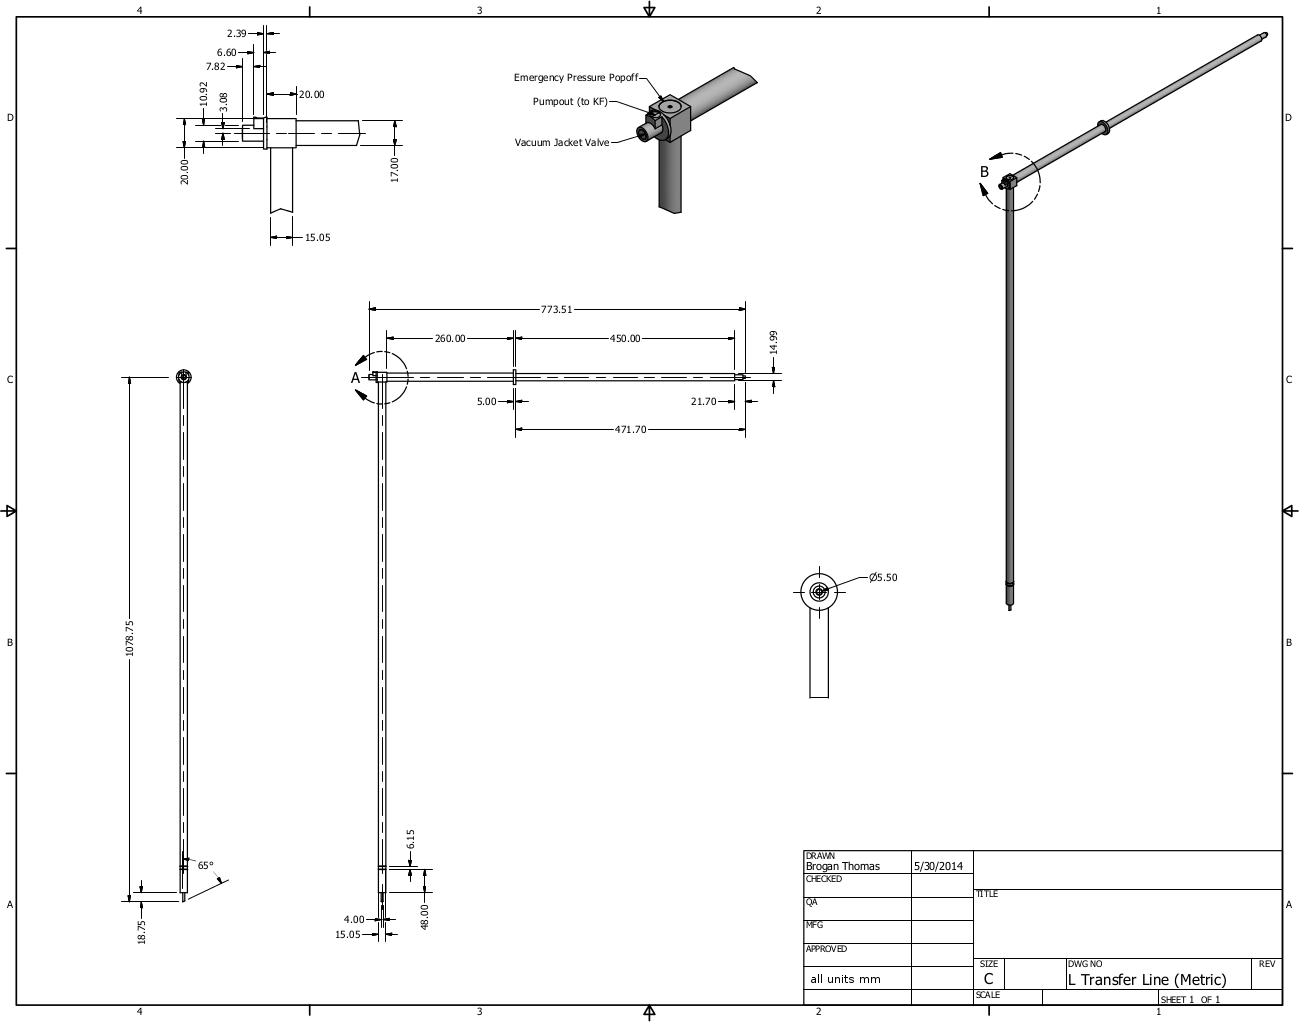
\includegraphics[width=\textwidth]{./img/LTL-drawing.png}
 \caption{Drawing of the LTL.}
 \label{fig:LTL-drawing}
\end{figure}

\begin{figure}[tbp!]
 \centering
 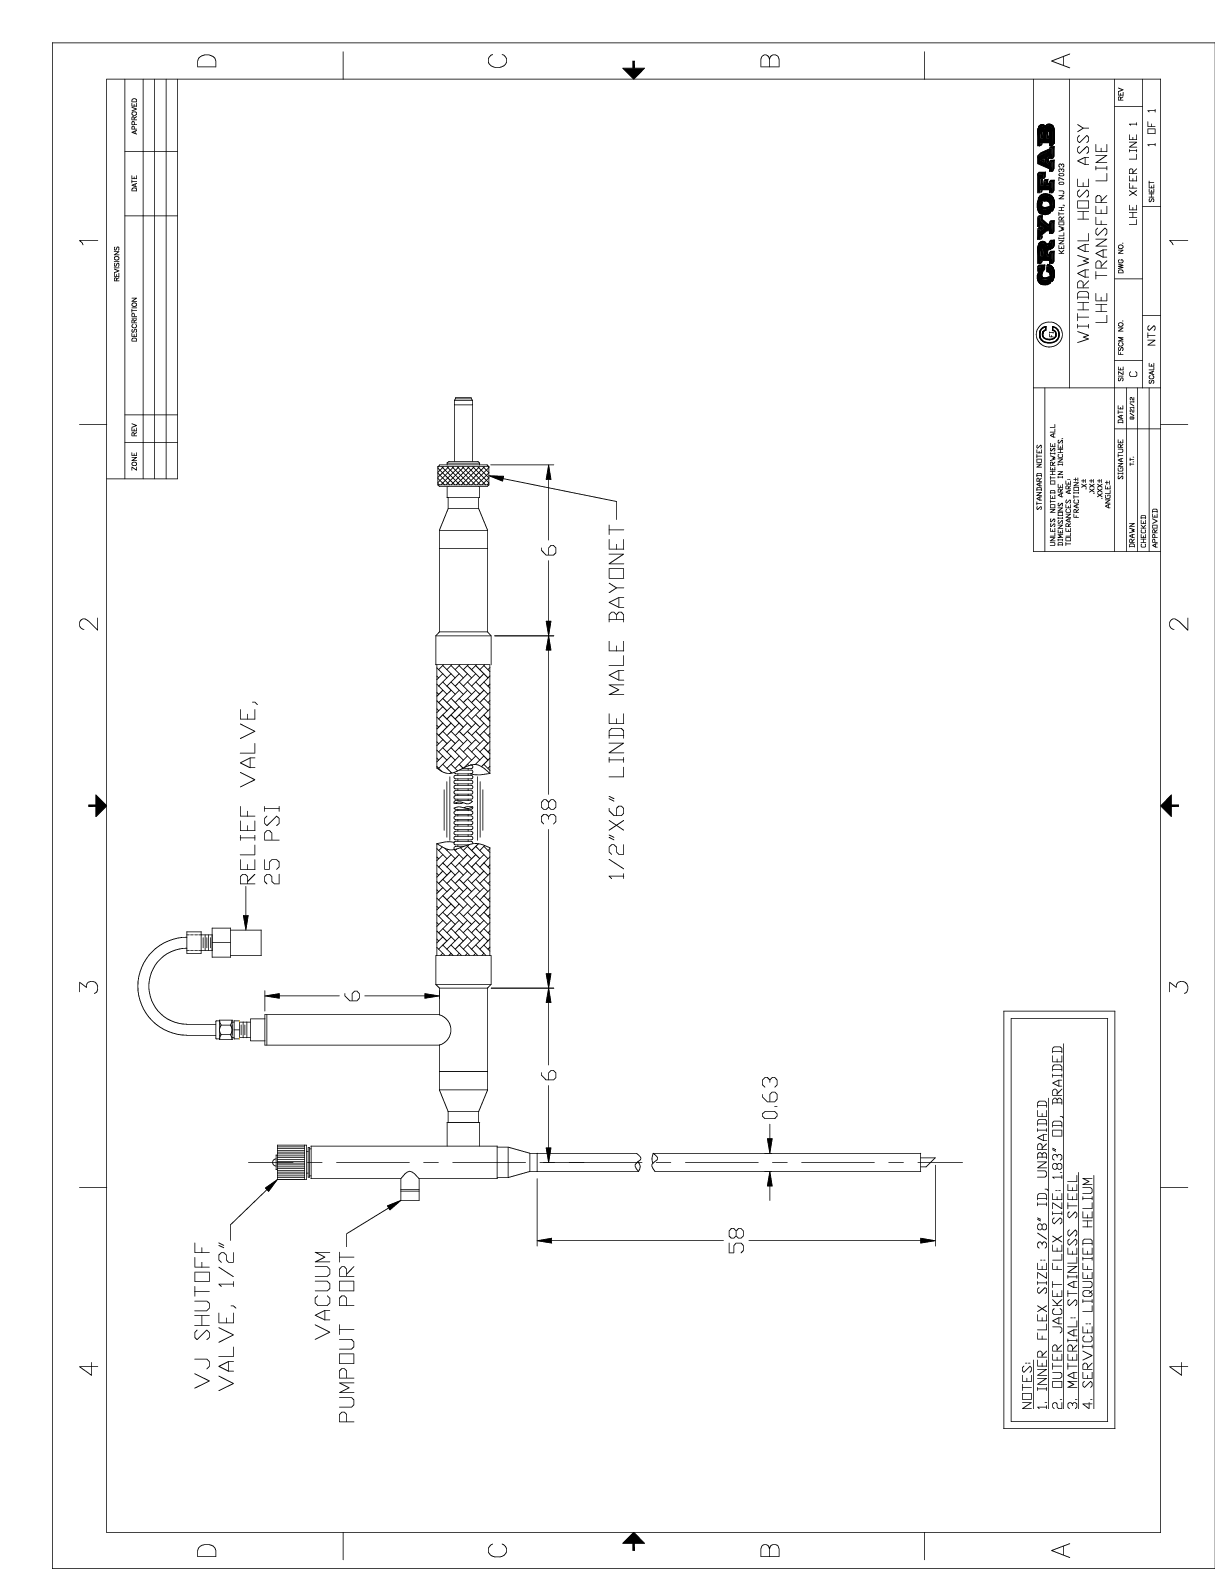
\includegraphics[width=\textwidth]{./img/500TL-drawing.png}
 \caption{Drawing of the 500TL.}
 \label{fig:500TL-drawing}
\end{figure}

\begin{figure}[tbp!]
 \centering
 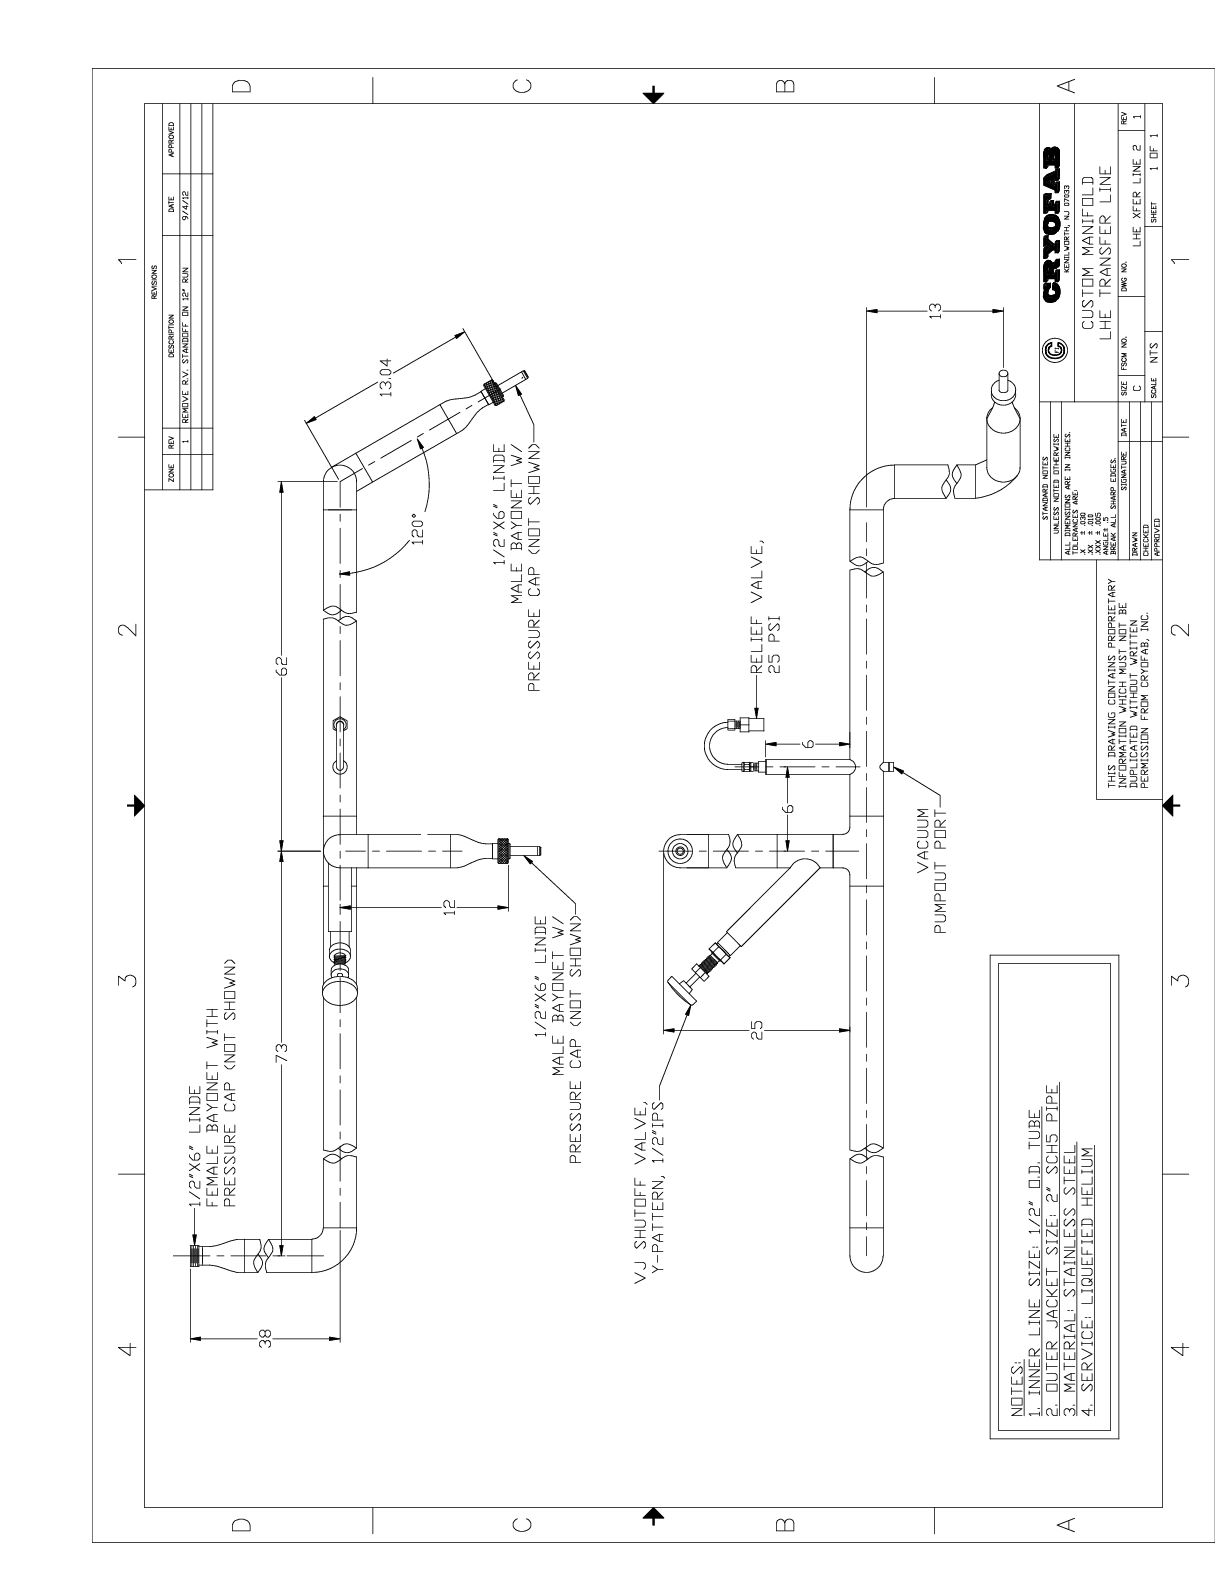
\includegraphics[width=\textwidth]{./img/WTL-drawing.png}
 \caption{Drawing of the WTL.}
 \label{fig:WTL-drawing}
\end{figure}

\begin{figure}[tbp!]
 \centering
 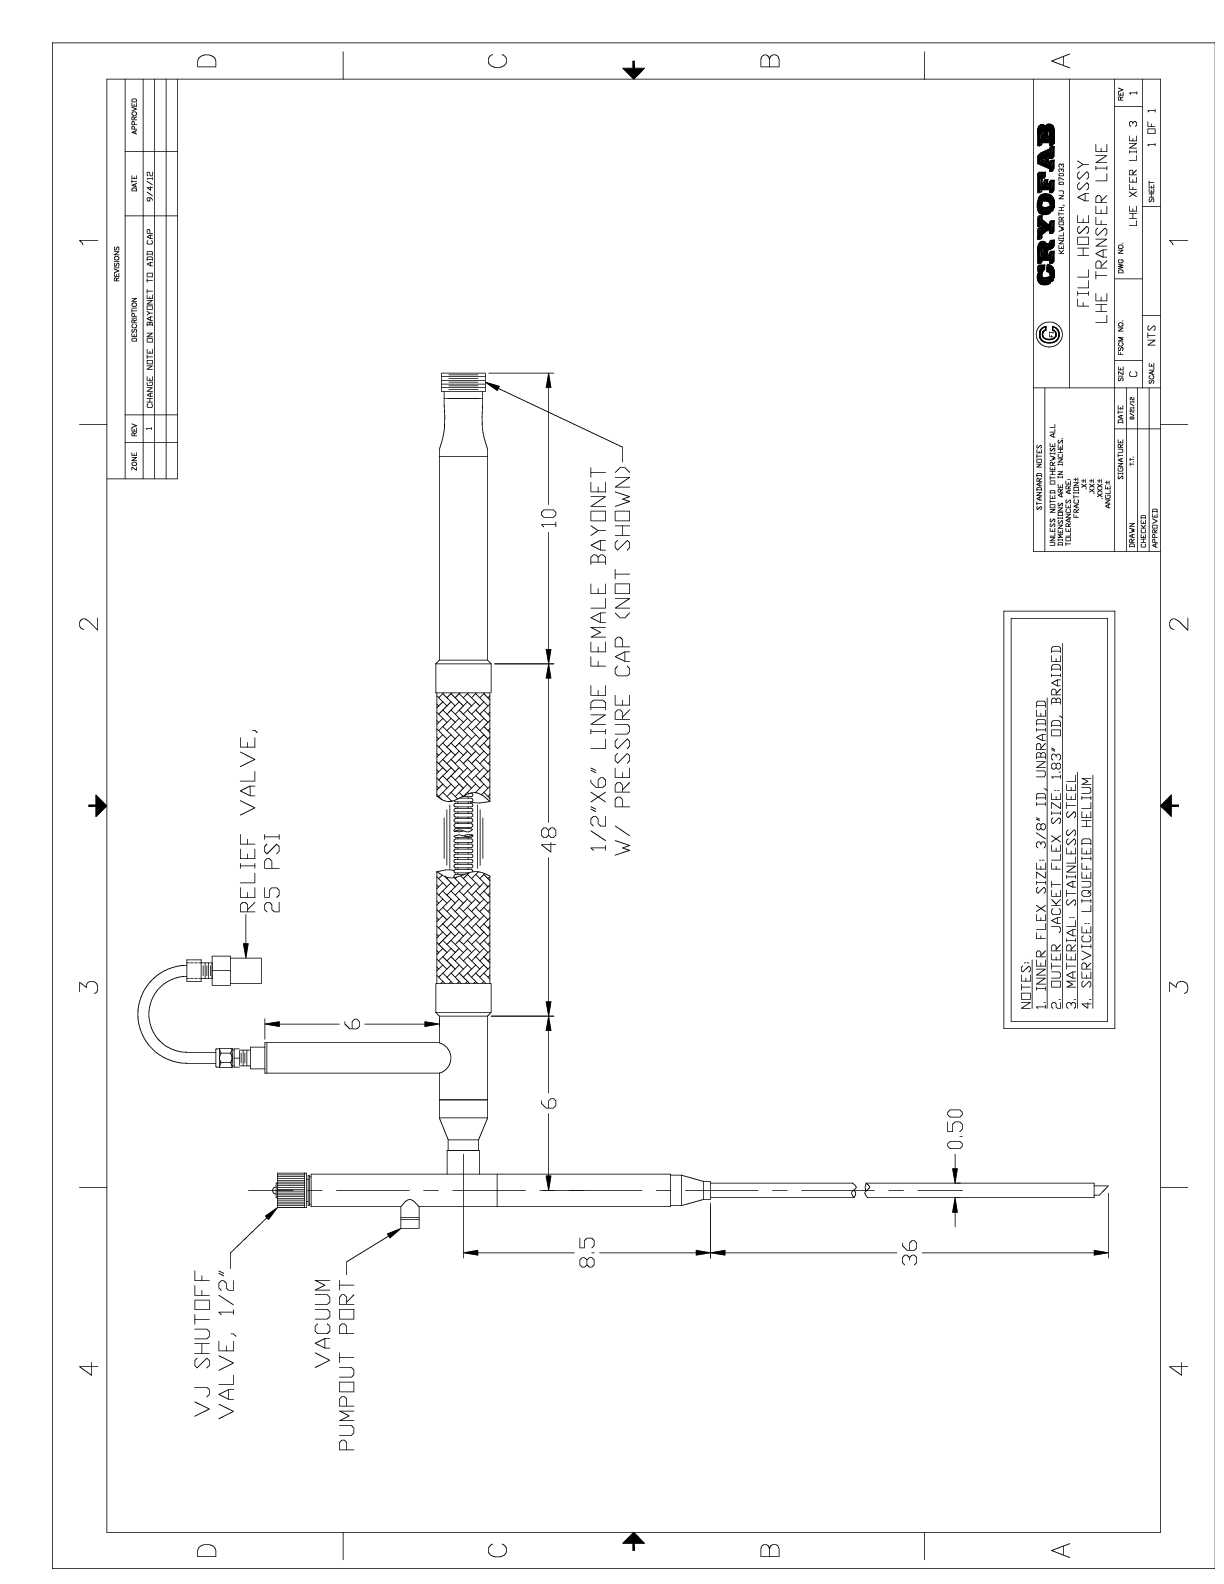
\includegraphics[width=\textwidth]{./img/MTL-drawing.png}
 \caption{Drawing of the MTL.}
 \label{fig:MTL-drawing}
\end{figure}

\begin{figure}[tbp!]
 \centering
 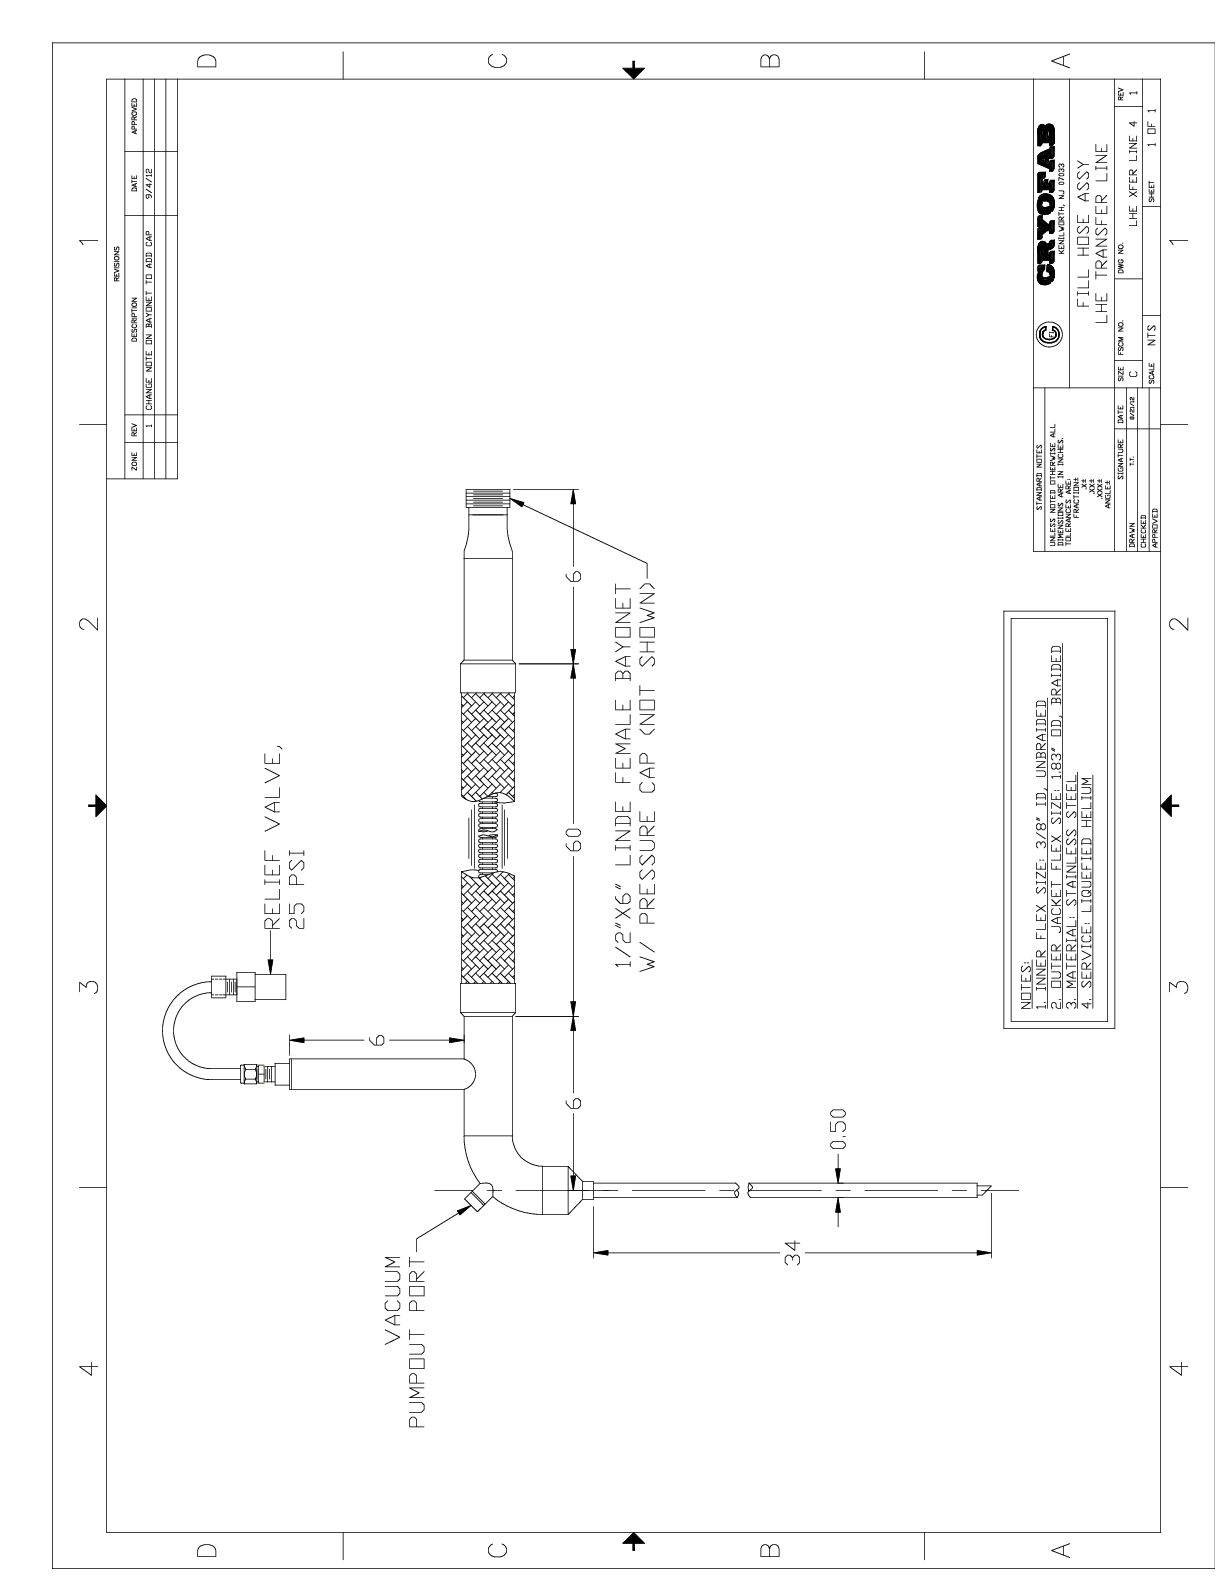
\includegraphics[width=\textwidth]{./img/100TL-drawing.png}
 \caption{Drawing of the 100TL.}
 \label{fig:100TL-drawing}
\end{figure}
\end{appendices}